\subsubsection{Job Creation Page Specifications}
The jobs page is where the user will select parameters and inputs, and queue jobs to be processed on their server instance. These jobs and their outputs are then stored in the local database, again either on the local machine or the server, if that is how the user is running the service. The functionality is as follows:\\
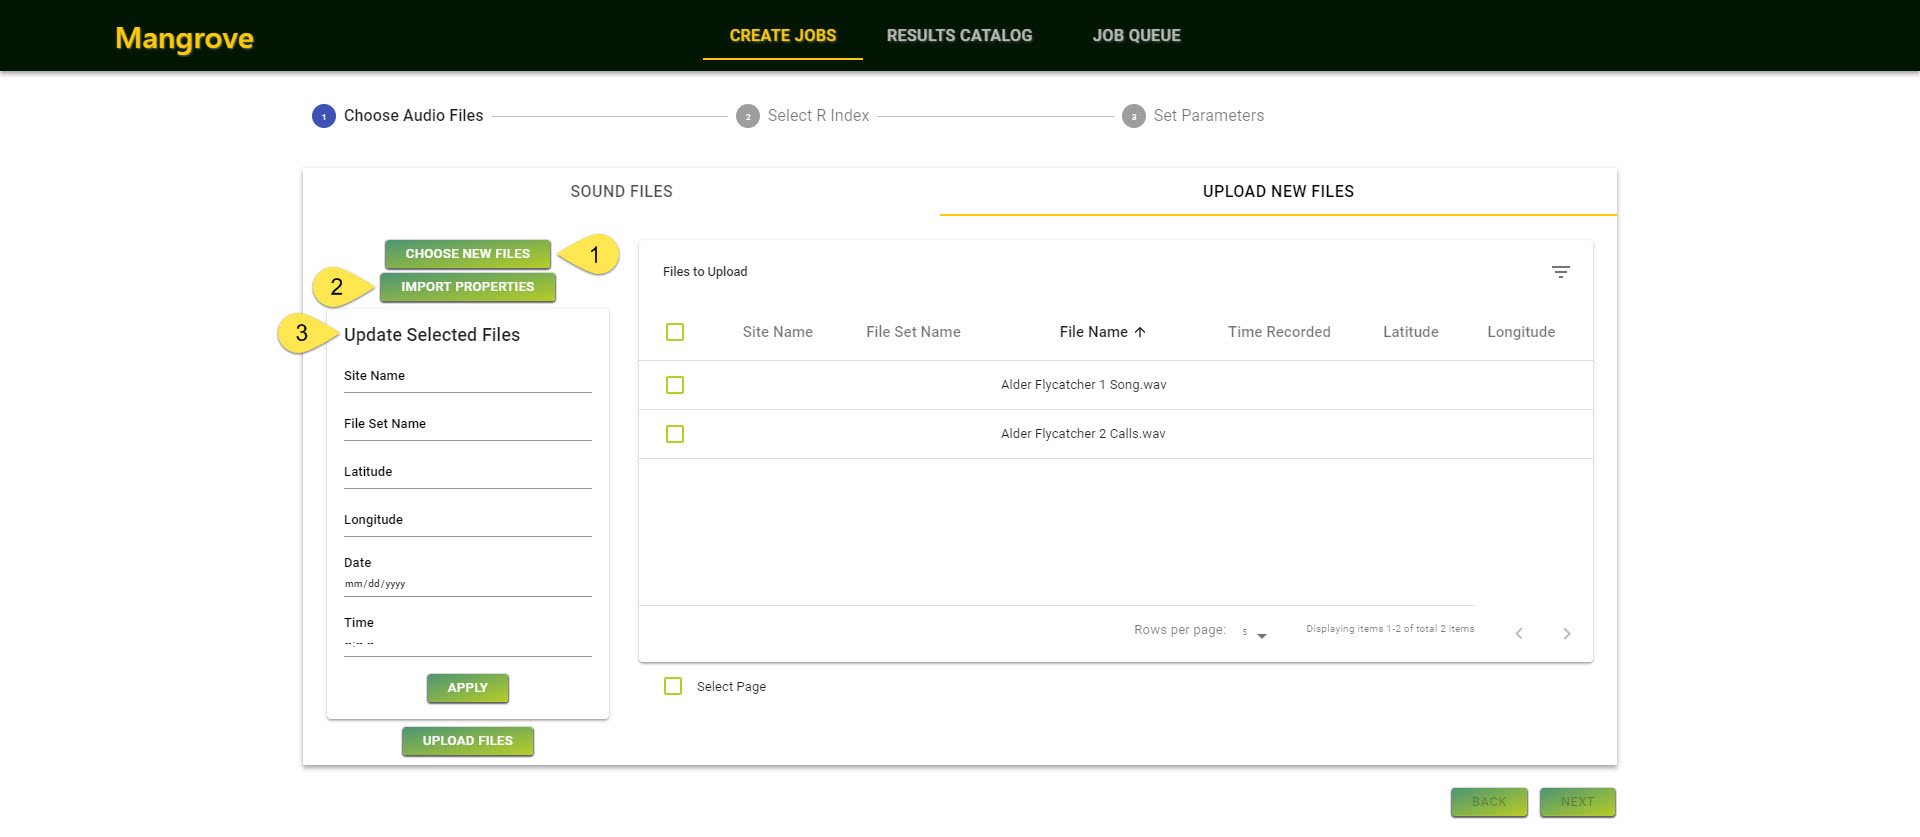
\includegraphics[width=\textwidth]{jobsPage-1}\\
Initially, users will need to upload files. The functionality of this step is outlined below:\\
\begin{enumerate}
  \item \textbf{Choose New Files}\\ This button will open up the user OS file explorer, and let them choose the input wav files they wish to add to their database.
  \item \textbf{Import Properties}\\ This button will allow the user to define file name format to automatically populate certain parts of the file metadata. This is especially useful for populating the file date field.
  \item \textbf{Inputting Metadata}\\ For each selected file in the table, you can input a Site and Series. This is essential to efficiently organizing user data and getting the most out of the analysis graphs. Additionally, the user must input the date and time the file was recorded, and the latitude and longitude optionally.
\end{enumerate}
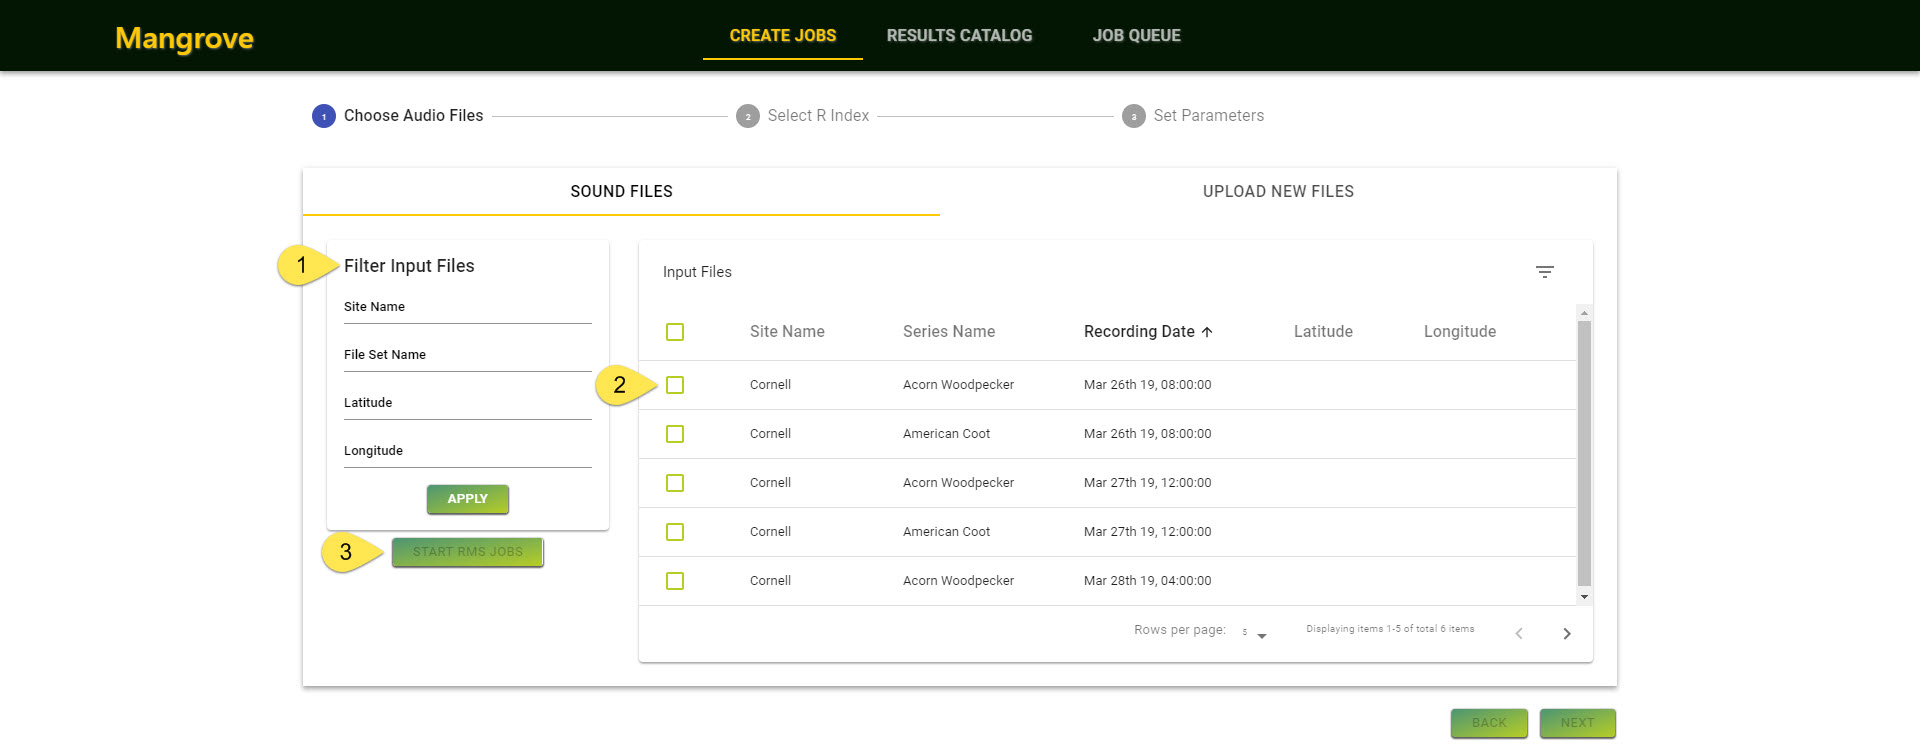
\includegraphics[width=\textwidth]{jobsPage-1-2}\\
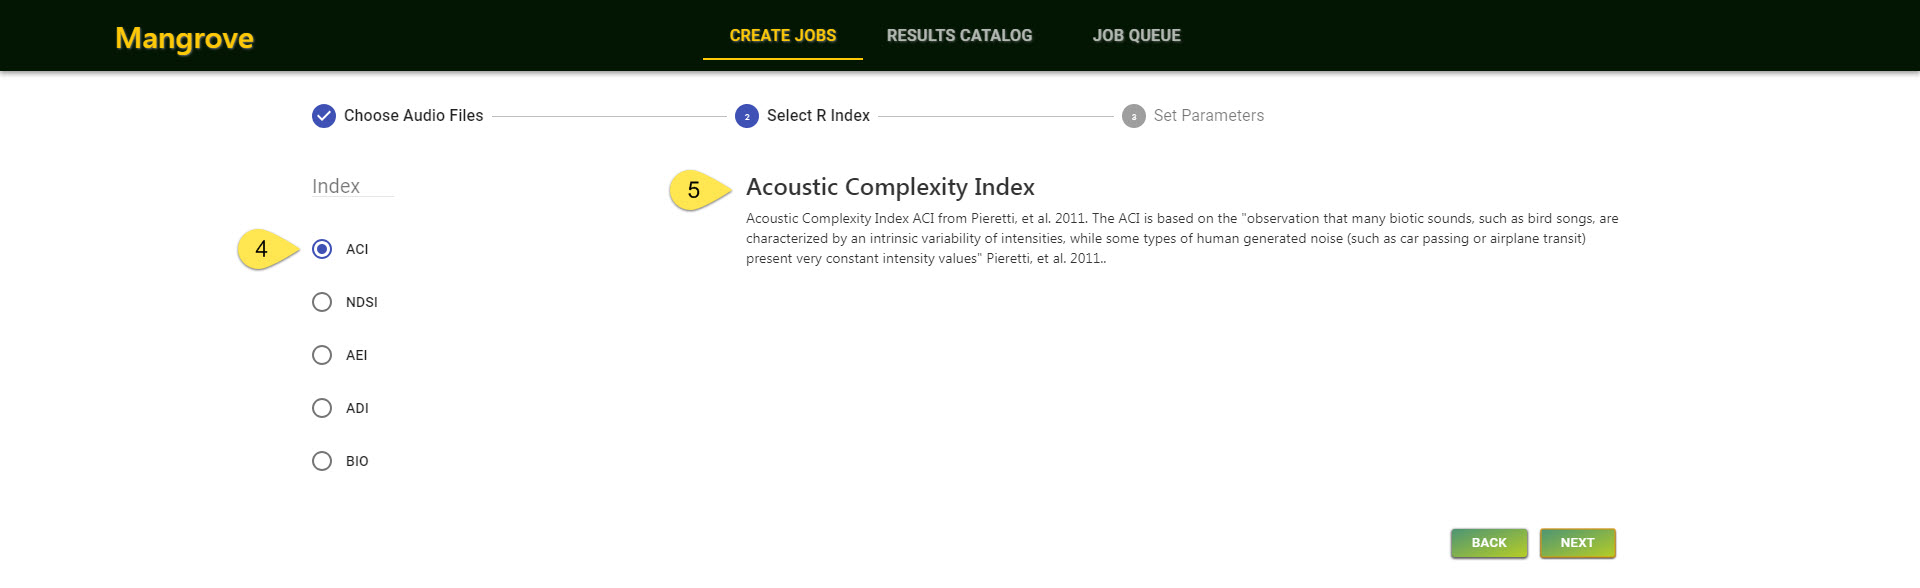
\includegraphics[width=\textwidth]{jobsPage-2}\\
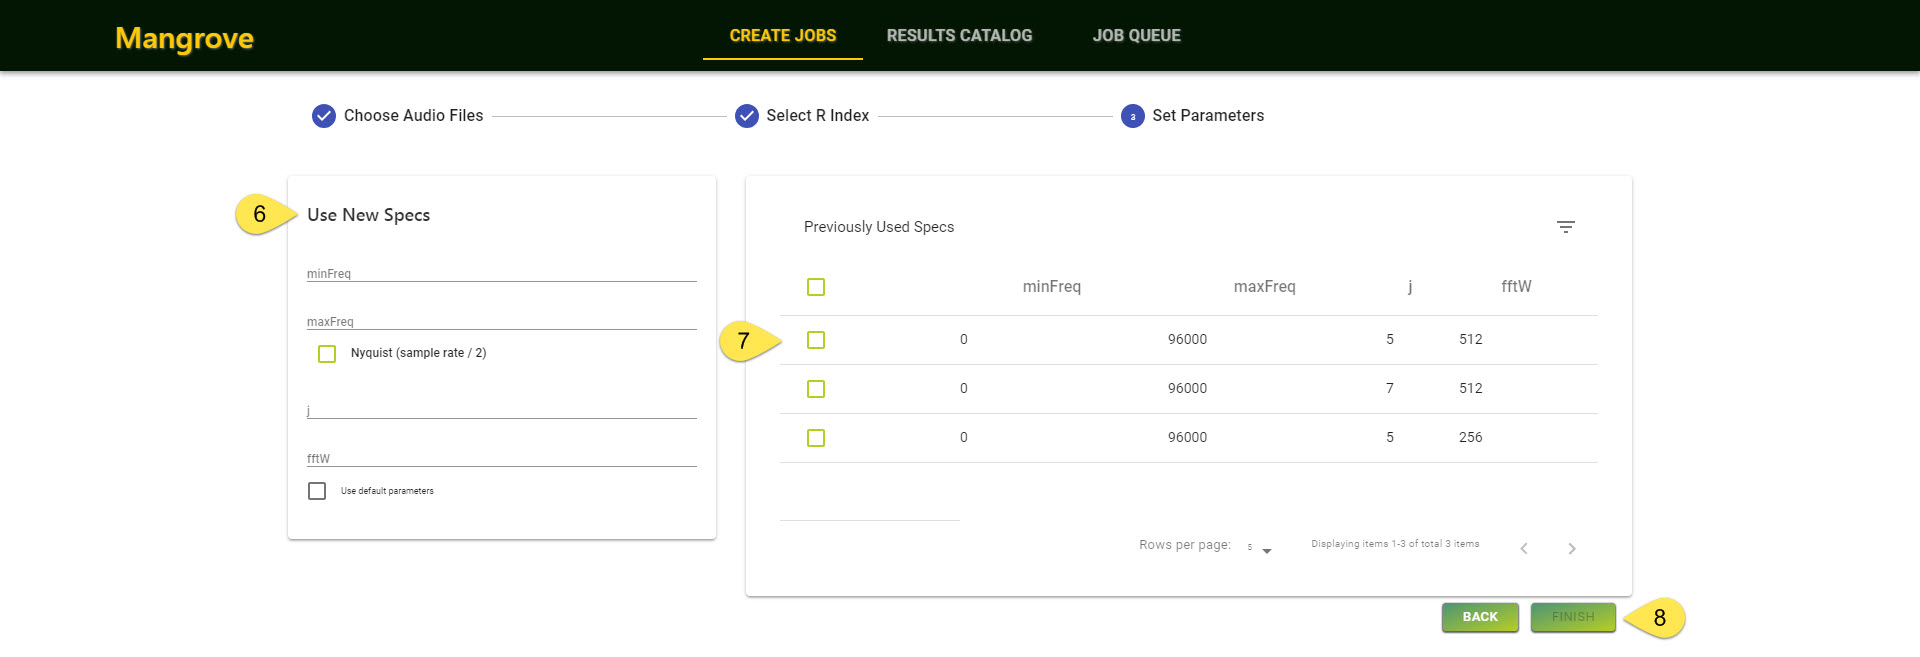
\includegraphics[width=\textwidth]{jobsPage-3}\\
As the user works with Mangrove, they will accumulate input files in their database. If the user wants to just use these files, they will take the following steps:\\
\begin{enumerate}
  \item \textbf{Filter Input Files}\\ Using this section, the user can define Sites and Series to filter inputs by. Additionally, they can define latitude and longitude coordinates to filter by as well.
  \item \textbf{Selecting Input Files}\\ This table will be populated with all files in the user\textquotesingle s database. If they have filtered them, only the filtered inputs will be shown. Using the checkboxes, the user will select all inputs they wish to run the job in in the coming sections.
  \item \textbf{Start RMS Jobs}\\ This button will auto start RMS index jobs on the selected inputs. The RMS index does not need any parameters and completes quite quickly, so this is more of a quick start option for this index.
  \item \textbf{Select Index}\\ This step includes selecting the index the user wishes to run. Each index aims to explore different information about a sound file, and the workings of them are explained in greater detail in the Soundscape Ecology Indices section of this paper.
  \item \textbf{Index Description}\\ A description of the selected index from research papers appears to help explain what each index does in order to aid the researcher when selecting which index to run.
  \item \textbf{Creating Specs}\\ Initially when the user begins working with Mangrove they will need to define specs to run jobs with. Each index has different parameters to run with, and the selected index will change what parameters appear in this section. There is a checkbox to use default parameters as well, these are defined in the R package being used to run these indices.
  \item \textbf{Selecting Specs}\\ Here, the newly created or already existing specs will appear. Using the checkboxes, the user will select the spec(s) they wish to use to run jobs on. This table can be sorted as well by parameter.
  \item \textbf{Finish}\\ Finally, selecting the Finish button will start these jobs and upload the jobs to the database. These jobs can be viewed in the Job Queue.
\end{enumerate}
